\documentclass[border=10pt]{standalone}

\usepackage{tikz}
\usepackage{tikzsymbols}
\usetikzlibrary{calc,patterns,shapes.geometric}

\def\centerarc[#1](#2)(#3:#4:#5){\draw[#1] ($(#2)+({#5*cos(#3)},{#5*sin(#3)})$) arc (#3:#4:#5);}

\begin{document}
	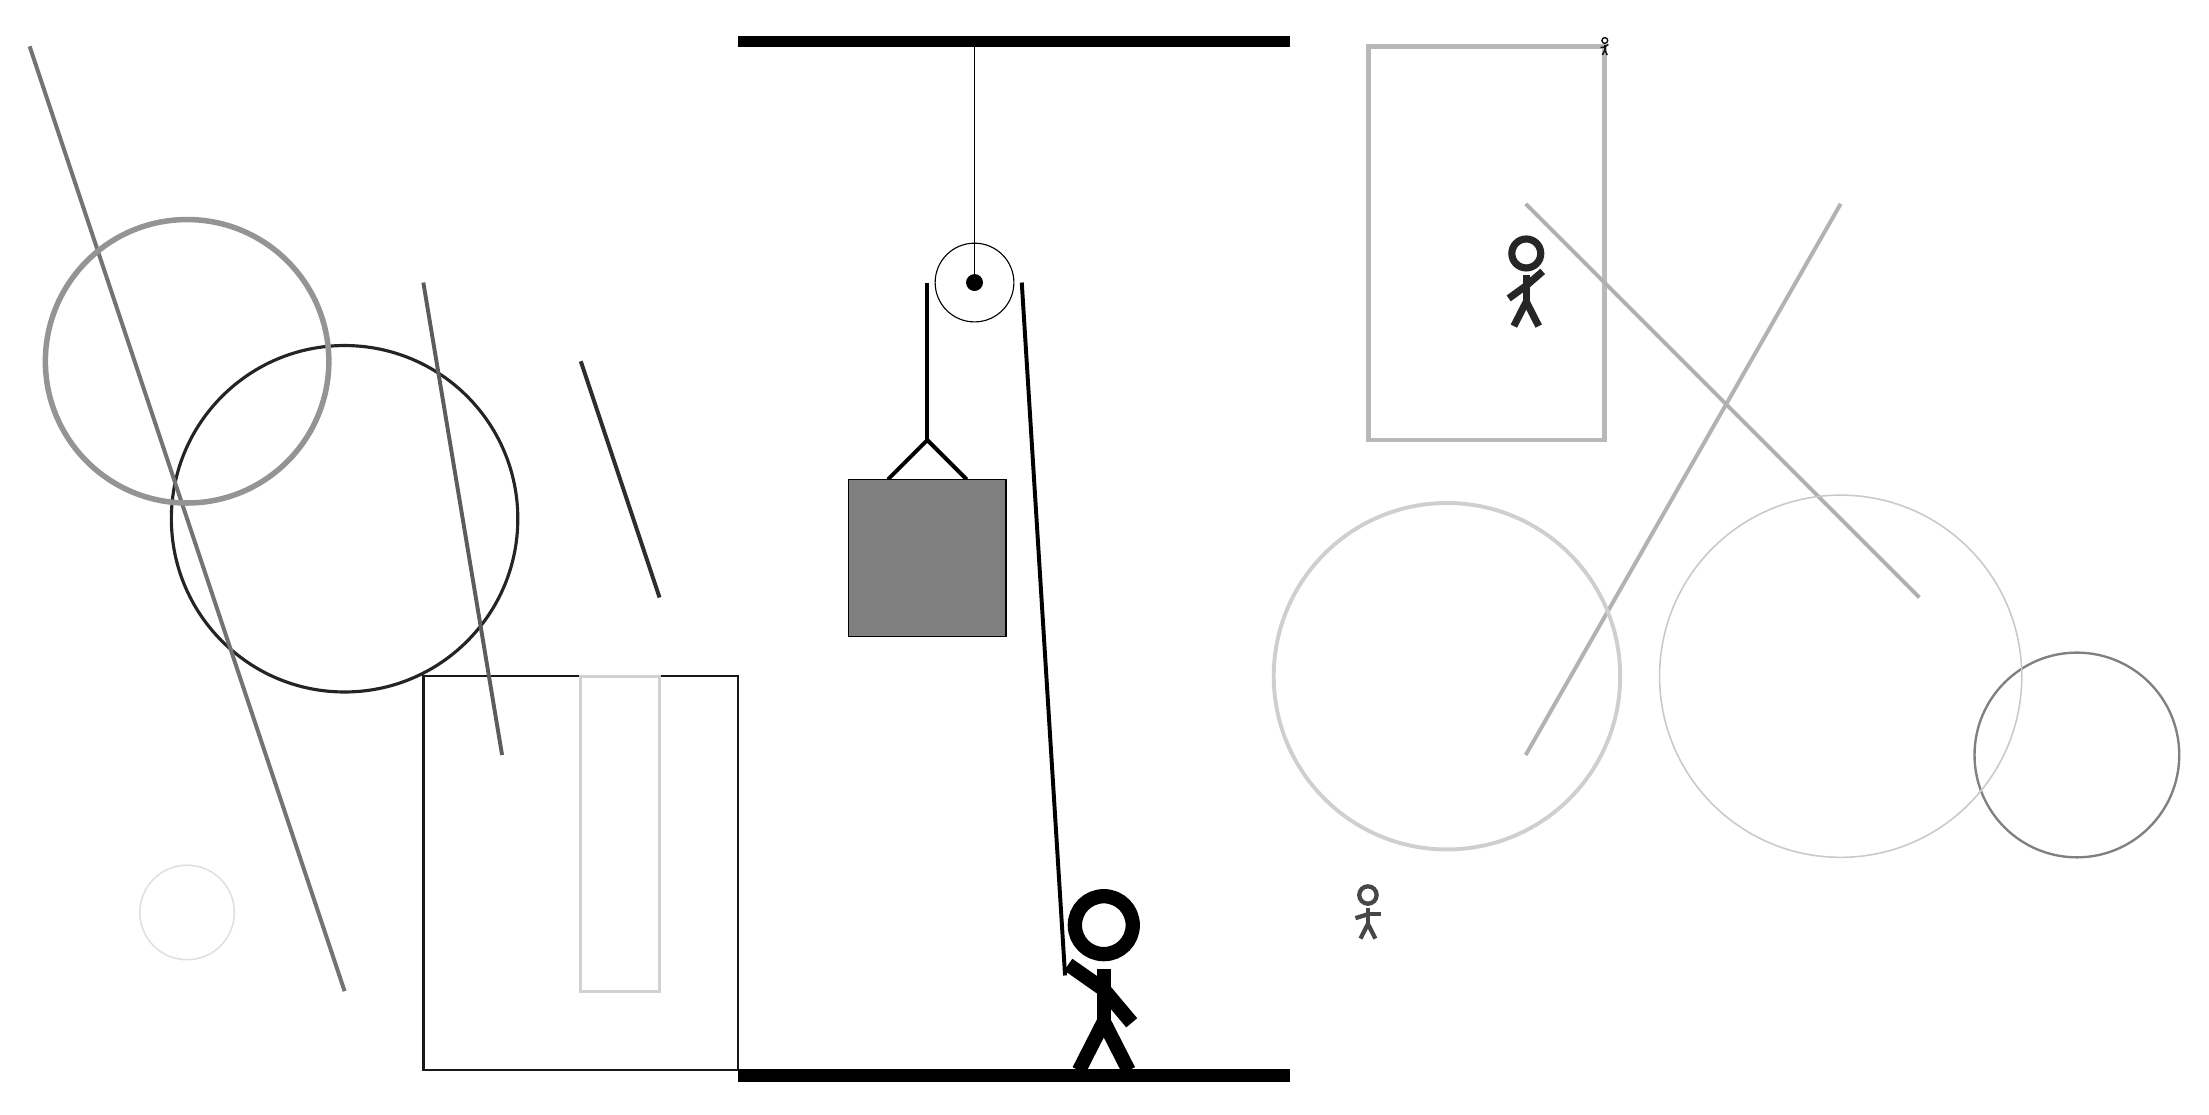
\begin{tikzpicture}
		%%%%% START %%%%%
		
		\draw[fill=black] (-2, 10) rectangle (5, 10.125);
		
		\draw (1, 7) circle (0.5);
		\draw[fill=black] (1, 7) circle (0.1);
		\draw (1, 10) -- (1, 7);
		
		\draw[line width=0.5mm] (-0.1, 4.5) -- (0.4, 5.0) -- (0.9, 4.5);
		\draw[fill=black!50] (-0.6, 4.5) rectangle (1.4, 2.5);
		
		\draw[line width=0.5mm] (0.4, 7) -- (0.4, 5.0);
		\centerarc[line width=0.5mm](1, 7)(0:180:0.6);
		\draw[line width=0.5mm](1.6, 7) -- (2.15, -1.8);
		
		\node at (2.6, -1.9) {\Strichmaxerl[10][-35][-50]};
		
		\node[line width=0.2mm, color=black!72] at (6, -1) {\Strichmaxerl[3][17][0]};
		
		\draw[line width=0.5mm, color=black!30](8, 1) -- (12, 8);
		\draw [line width=0.4mm, color=black!86](-7, 4) circle (2.2);
		\draw[line width=0.6mm, color=black!28] (6, 5) rectangle (9, 10);
		\draw [line width=0.5mm, color=black!19](7, 2) circle (2.2);
		\node[line width=0.3mm, color=black!92] at (9, 10) {\Strichmaxerl[1][8][35]};
		\draw[line width=0.5mm, color=black!55](-7, -2) -- (-11, 10);
		\node[line width=0.6mm, color=black!85] at (8, 7) {\Strichmaxerl[5][36][41]};
		\draw[line width=0.3mm, color=black!90] (-2, 2) rectangle (-6, -3);
		\draw[line width=0.5mm, color=black!64](-6, 7) -- (-5, 1);
		
		\draw[line width=0.4mm, color=black!18] (-4, -2) rectangle (-3, 2);
		
		\draw[line width=0.5mm, color=black!82](-3, 3) -- (-4, 6);
		\draw[line width=0.5mm, color=black!31](8, 8) -- (13, 3);
		\draw [line width=0.2mm, color=black!12](-9, -1) circle (0.6);
		\draw [line width=0.3mm, color=black!50](15, 1) circle (1.3);
		\draw [line width=0.2mm, color=black!21](12, 2) circle (2.3);
		
		\draw [line width=0.7mm, color=black!42](-9, 6) circle (1.8);
		
		\draw[fill=black] (-2, -3) rectangle (5, -3.15);
		
		%%%%% END %%%%%
	\end{tikzpicture}
\end{document}